\documentclass[10pt, a4paper]{jsarticle}
\usepackage[dvipdfm]{graphicx}
\usepackage{otf}
\usepackage{amsmath}
\usepackage{listings,jvlisting} %日本語のコメントアウトをする場合jvlisting(もしくはjlisting)が必要
%ここからソースコードの表示に関する設定
\lstset{
  basicstyle={\ttfamily},
  identifierstyle={\small},
  commentstyle={\smallitshape},
  keywordstyle={\small\bfseries},
  ndkeywordstyle={\small},
  stringstyle={\small\ttfamily},
  frame={tb},
  breaklines=true,
  columns=[l]{fullflexible},
  numbers=left,
  xrightmargin=0zw,
  xleftmargin=3zw,
  numberstyle={\scriptsize},
  stepnumber=1,
  numbersep=1zw,
  lineskip=-0.5ex,
  keepspaces=true,
}
\title{複雑系科学演習 第2回 レポート} % タイトルを決める作業
\begin{document} % 文書の始まり
\author{複雑系知能学科 複雑系コース 3年 Iクラス番号1019086 岩上慎之介}
\maketitle % 決めたタイトルを挿入する作業
\newpage
% \tableofcontents
\section{レポート課題 1st}

\subsection{課題1}
前頁の関数nextをテント写像に書き換え,リターンマップを描け\\
\subsubsection{画像}
\begin{figure}[htbp]
  \centering
  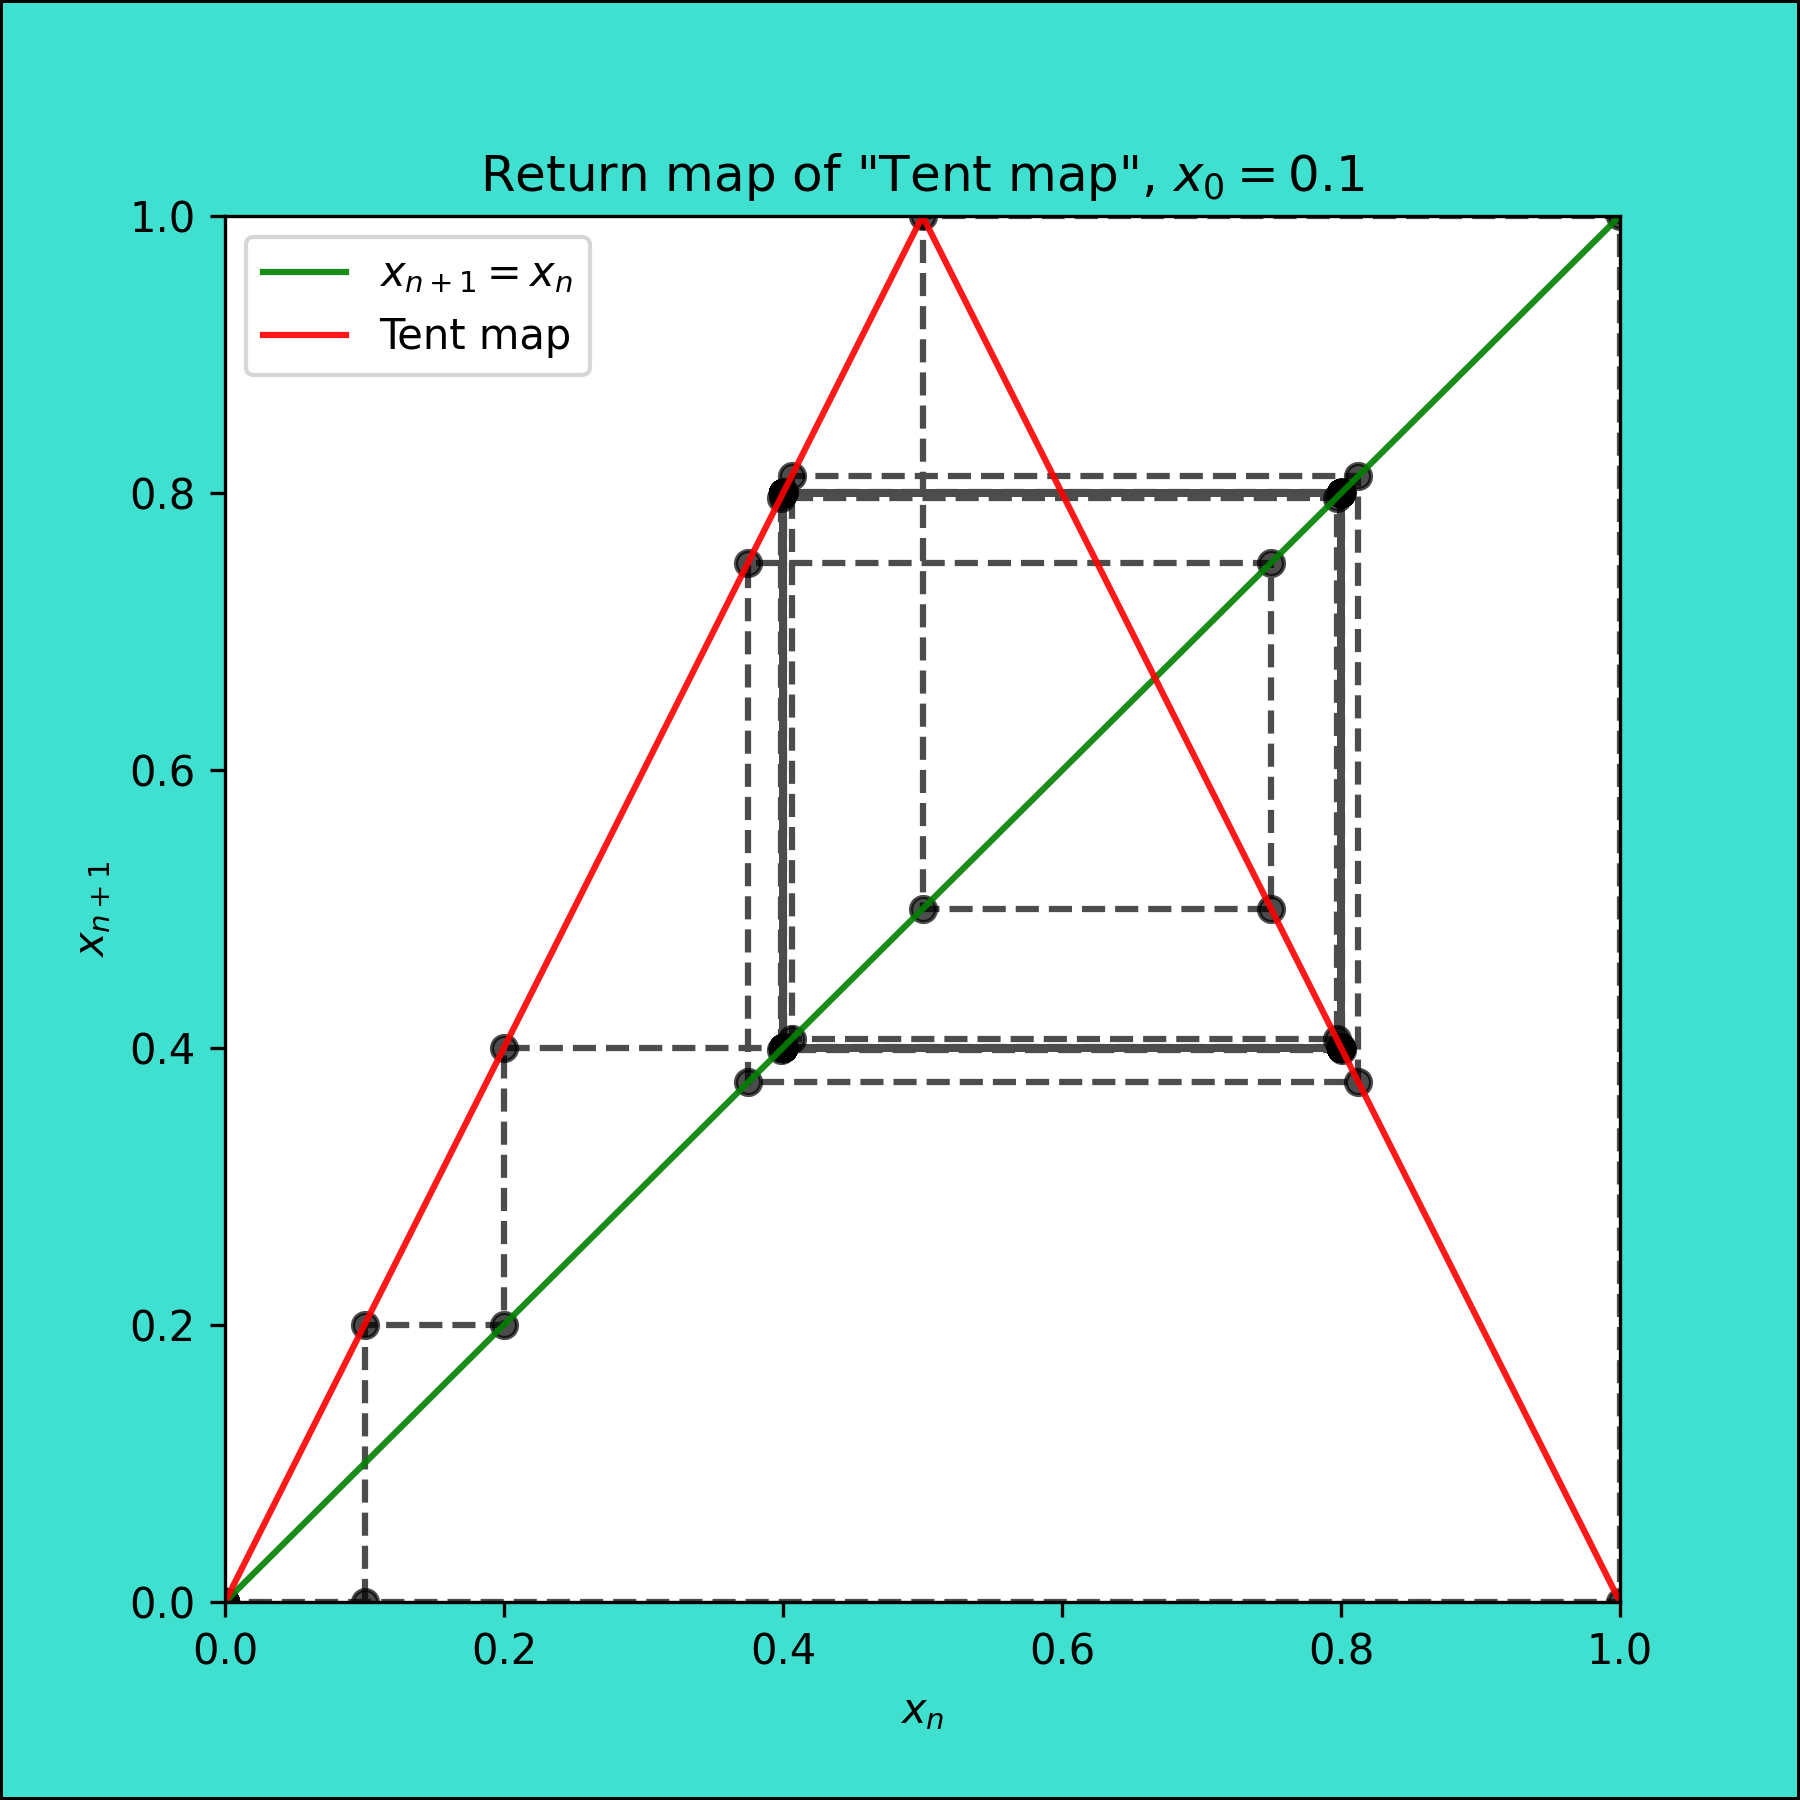
\includegraphics[keepaspectratio, scale=0.7]{images/Problem6/task6.png}
\end{figure}

\subsubsection{ソースコード}
\begin{lstlisting}[caption=task6]
  from matplotlib import pyplot as plt
  import numpy as np


  class Task6():
      def __init__(self) -> None:
          self.x = 0.1                      # 初期値 x0 = 0.1
          self.xn = np.linspace(0, 1, 1000)  # 横軸の範囲と刻み幅
          self.tent_y = []                  # テント写像のグラフを描くための配列
          for i in self.xn:
              if 0 <= i <= 0.5:
                  self.tent_y.append(2 * i)
              else:
                  self.tent_y.append(2 * (1 - i))
          self.filepath = '複雑系科学演習/Week6/images/task6'

      def tent(self) -> list:
          "リターンマップでのテント写像の座標を持つ配列を返す"
          calc_x = self.x
          x_array = [calc_x]
          for _ in range(100):
              if 0 <= calc_x <= 0.5:
                  calc_x = 2 * calc_x
              else:
                  calc_x = 2 * (1 - calc_x)
              x_array.append(calc_x)
          return x_array

      def plot_return_map(self) -> None:
          "リターンマップの描画(テント写像)"
          plt.figure(figsize=(6, 6), facecolor='turquoise',
                    linewidth=1, edgecolor='black')
          n = self.tent()
          spiper_plot_x = [self.x]          # クモの巣図用の配列(x)
          spiper_plot_y = [0]               # クモの巣図用の配列(y)
          for i in range(1, len(n)):
              spiper_plot_x.append(n[i - 1])
              spiper_plot_x.append(n[i])
              spiper_plot_y.append(n[i])
              spiper_plot_y.append(n[i])

          plt.plot(spiper_plot_x, spiper_plot_y, marker='o',
                  linestyle='dashed', color='black', alpha=0.7)
          plt.plot(self.xn, self.xn, color='green',
                  alpha=0.9, label="$x_{n+1} = x_n$")
          plt.plot(self.xn, self.tent_y, color='red',
                  alpha=0.9, label="Tent map")
          plt.title("Return map of \"Tent map\", $x_0 = $" + str(self.x))
          plt.xlim(0, 1)
          plt.ylim(0, 1)
          plt.xlabel("$x_n$")
          plt.ylabel("$x_{n+1}$")
          plt.legend(loc='best')
          plt.savefig(self.filepath, dpi=300)


  task = Task6()
  task.plot_return_map()
\end{lstlisting}


\subsection{課題2}
$x_0 = \dfrac{1}{10}$ として、どのような周期解になるか厳密にて計算せよ。\\\\
手計算で $x_i$ の値を計算すると、
\begin{equation}
  \begin{split}
    x_0& = \dfrac{1}{10}\\
    x_1& = 2 \times \dfrac{1}{10} = \dfrac{1}{5}\\
    x_2& = 2 \times \dfrac{1}{5} = \dfrac{2}{5}\\
    x_3& = 2 \times \dfrac{2}{5} = \dfrac{2}{5}\\
    x_4& = 2 \times \left( 1 - \dfrac{4}{5} \right) = \dfrac{2}{5}\\
    x_5& = 2 \times \dfrac{2}{5} = \dfrac{2}{5}\\
    x_6& = 2 \times \left( 1 - \dfrac{4}{5} \right) = \dfrac{2}{5}\\
    .\\.\\.
  \end{split}
\end{equation}
となるため $\dfrac{2}{5}$ と $\dfrac{4}{5}$ の2つの周期解(2周期解)を取り続けていく。

\subsection{課題3}
$x_0 = \dfrac{1}{10}$ として、前のプログラムを実行せよ。ただし $N = 100$ とし $x_{100}$ まで数値計算せよ。どのような結果となったか。理由も述べよ。

\subsubsection{出力}
\begin{lstlisting}[caption=out]
  0.700000 0.600000
  0.600000 0.600000
  0.600000 0.800000
  0.800000 0.800000
  0.800000 0.400000
  0.400000 0.400000
  0.400000 0.800000
  0.800000 0.800000
  0.800000 0.400000
  0.400000 0.400000
  0.400000 0.800000
  0.800000 0.800000
  0.800000 0.400000
  0.400000 0.400000
  0.400000 0.800000
  0.800000 0.800000
  0.800000 0.400000
  0.400000 0.400000
  0.400000 0.800000
  0.800000 0.800000
  0.800000 0.400000
  0.400000 0.400000
  0.400000 0.800000
  0.800000 0.800000
  0.800000 0.400000
  0.400000 0.400000
  0.400000 0.800000
  0.800000 0.800000
  0.800000 0.400000
  0.400000 0.400000
  0.400000 0.800000
  0.800000 0.800000
  0.800000 0.400000
  0.400000 0.400000
  0.400000 0.800000
  0.800000 0.800000
  0.800000 0.400000
  0.400000 0.400000
  0.400000 0.800000
  0.800000 0.800000
  0.800000 0.400000
  0.400000 0.400000
  0.400000 0.800000
  0.800000 0.800000
  0.800000 0.400000
  0.400000 0.400000
  0.400000 0.800000
  0.800000 0.800000
  0.800000 0.400000
  0.400000 0.400000
  0.400000 0.800000
  0.800000 0.800000
  0.800000 0.400000
  0.400000 0.400000
  0.400000 0.800000
  0.800000 0.800000
  0.800000 0.400000
  0.400000 0.400000
  0.400000 0.800000
  0.800000 0.800000
  0.800000 0.400000
  0.400000 0.400000
  0.400000 0.800000
  0.800000 0.800000
  0.800000 0.400000
  0.400000 0.400000
  0.400000 0.799999
  0.799999 0.799999
  0.799999 0.400002
  0.400002 0.400002
  0.400002 0.800003
  0.800003 0.800003
  0.800003 0.399994
  0.399994 0.399994
  0.399994 0.799988
  0.799988 0.799988
  0.799988 0.400024
  0.400024 0.400024
  0.400024 0.800049
  0.800049 0.800049
  0.800049 0.399902
  0.399902 0.399902
  0.399902 0.799805
  0.799805 0.799805
  0.799805 0.400391
  0.400391 0.400391
  0.400391 0.800781
  0.800781 0.800781
  0.800781 0.398438
  0.398438 0.398438
  0.398438 0.796875
  0.796875 0.796875
  0.796875 0.406250
  0.406250 0.406250
  0.406250 0.812500
  0.812500 0.812500
  0.812500 0.375000
  0.375000 0.375000
  0.375000 0.750000
  0.750000 0.750000
  0.750000 0.500000
  0.500000 0.500000
  0.500000 1.000000
  1.000000 1.000000
  1.000000 0.000000
  0.000000 0.000000
  0.000000 0.000000
  0.000000 0.000000
  0.000000 0.000000
  0.000000 0.000000
  0.000000 0.000000
  0.000000 0.000000
  0.000000 0.000000
  0.000000 0.000000
  0.000000 0.000000
  0.000000 0.000000
  0.000000 0.000000
  0.000000 0.000000
  0.000000 0.000000
  0.000000 0.000000
  0.000000 0.000000
  0.000000 0.000000
  0.000000 0.000000
  0.000000 0.000000
  0.000000 0.000000
  0.000000 0.000000
  0.000000 0.000000
  0.000000 0.000000
  0.000000 0.000000
  0.000000 0.000000
  0.000000 0.000000
  0.000000 0.000000
  0.000000 0.000000
  0.000000 0.000000
  0.000000 0.000000
  0.000000 0.000000
  0.000000 0.000000
  0.000000 0.000000
  0.000000 0.000000
  0.000000 0.000000
  0.000000 0.000000
  0.000000 0.000000
  0.000000 0.000000
  0.000000 0.000000
  0.000000 0.000000
  0.000000 0.000000
  0.000000 0.000000
  0.000000 0.000000
  0.000000 0.000000
  0.000000 0.000000
  0.000000 0.000000
  0.000000 0.000000
  0.000000 0.000000
  0.000000 0.000000
  0.000000 0.000000
  0.000000 0.000000
  0.000000 0.000000
  0.000000 0.000000
  0.000000 0.000000
  0.000000 0.000000
  0.000000 0.000000
  0.000000 0.000000
  0.000000 0.000000
  0.000000 0.000000
  0.000000 0.000000
  0.000000 0.000000
  0.000000 0.000000
  0.000000 0.000000
  0.000000 0.000000
  0.000000 0.000000
  0.000000 0.000000
  0.000000 0.000000
  0.000000 0.000000
  0.000000 0.000000
  0.000000 0.000000
  0.000000 0.000000
  0.000000 0.000000
  0.000000 0.000000
  0.000000 0.000000
  0.000000 0.000000
  0.000000 0.000000
  0.000000 0.000000
  0.000000 0.000000
  0.000000 0.000000
  0.000000 0.000000
  0.000000 0.000000
  0.000000 0.000000
  0.000000 0.000000
  0.000000 0.000000
  0.000000 0.000000
  0.000000 0.000000
  0.000000 0.000000
  0.000000 0.000000
  0.000000 0.000000
  0.000000 0.000000
  0.000000 0.000000
  0.000000 0.000000
  0.000000 0.000000
  0.000000 0.000000
  0.000000 0.000000
  0.000000 0.000000
  0.000000 0.000000
\end{lstlisting}

\subsubsection{結果と考察}
実行した結果、$0.4$ と $0.8$ でずっとループすることはなく途中から値が変化した。最終的には、$(x_n, x_{n+1}) = (0, 0)$ を取り続けるようになった。これは、コンピュータの丸め誤差が影響し値が変化したと考えられる。
\subsubsection{ソースコード}
\begin{lstlisting}[caption=tent.c]
  #include<stdio.h>
  #define N 100
  double next(double x, double r) {
      if (0 <= x && x <= 0.5) {
          return 2 * x;
      } else {
          return 2 * (1 - x);
      }
  }
  int main(void){
      int n;
      double r;
      double xn = 0.7;
      double xn1;
      scanf("%lf", &r);
      for(n = 0; n <= N; n++) {
          xn1 = next(xn, r);
          printf("%lf %lf\n", xn, xn1);
          printf("%lf %lf\n", xn1, xn1);
          xn = xn1;
      }
      return 0;
  }
\end{lstlisting}

\subsection{課題4}
テント写像のリアプノフ指数を計算せよ。プログラミングが必要なければ手計算でよい。\\
リアプノフ指数 $\lambda$ は、\\
\begin{equation}
  \lambda = \lim_{n \to \infty} \dfrac{1}{n} \sum_{i = 0}^{n-1} \log |f'(x_i)|
\end{equation}
と表すことができる。\\
今回はテント写像のリアプノフ指数について調べていくので、関数 $f(x_i)$ は、
\begin{equation}
  f(x_i) =
    \begin{cases}
      2x_i & \left( 0 \leq x_i \leq \dfrac{1}{2} \right)\\
      2(1 - x_i) & \left( \dfrac{1}{2} < x_i \leq 1 \right)
    \end{cases}
\end{equation}
となる。さらに $(3)$ を用いて計算すると $f'(x_i)$は、
\begin{equation}
  f'(x_i) =
    \begin{cases}
      2 & \left( 0 \leq x_i \leq \dfrac{1}{2} \right)\\
      -2 & \left( \dfrac{1}{2} < x_i \leq 1 \right)
    \end{cases}
\end{equation}
となる。よって、$|f'(x_i)| = 2$ である。したがって、テント写像のリアプノフ指数 $\lambda$ は、
\begin{equation}
  \begin{split}
    \lambda& = \lim_{n \to \infty} \dfrac{1}{n} \sum_{i = 0}^{n-1} \log 2\\
    & = \lim_{n \to \infty} \dfrac{1}{n} \times n \log 2\\
    & = \lim_{n \to \infty} \log 2\\
    & = \log 2
  \end{split}
\end{equation}
と計算することができ $\lambda = \log 2$ となる。 

\subsection{課題5}
テント写像は $x_n$ から $x_{n+1}$ を求める写像である。 $y_n = \sin^2 \left( \dfrac{\pi}{2} x_n \right)$ と定義して、 $y_{n+1}$ を $y_n$ の式として表わせ。\\
\section{レポート課題 2nd}
\subsection{課題1}
\subsubsection{問題}
$r = 3.8285$ として、$x_n$ が$250 \leq n \leq 500$ の場合の時系列とリターンマップを描け、初期値は適当でよい。周期3を確認せよ(3周期の窓)
\subsubsection{画像}
\begin{figure}[htbp]
  \centering
  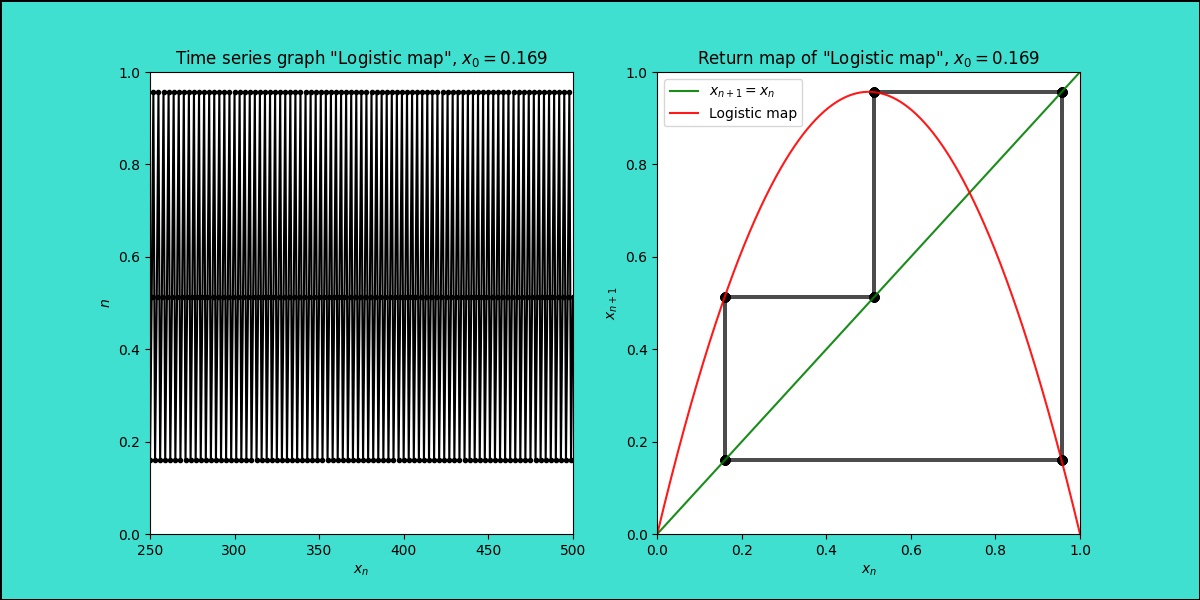
\includegraphics[keepaspectratio, scale=0.5]{images/Problem7/task7_1.png}
\end{figure}
\subsubsection{考察}
$r = 3.8285$ のときは、前回のレポート課題3に書いてあるロジスティック写像の分岐図を見ると、3周期解になっている範囲だとわかる。実際にグラフを描くと、時系列グラフ、リターンマップともに3つの解で周期性を持っていることが読み取れた。また、初期値をランダムにとって複数回プログラムを実行してもどちらのグラフにも変化は見られなかった。よって、$r = 3.8285$ のときはカオスの条件には当てはまらず周期性(3周期)を持っていると考察した。

\newpage
\subsection{課題2}
\subsubsection{問題}
$r = 3.8284$ として、$x_n$ が$250 \leq n \leq 500$ の場合の時系列とリターンマップを描け、初期値は適当でよい。規則的な部分(ラミナー)と不規則の部分(バースト)を確認せよ。
\subsubsection{画像}
\begin{figure}[htbp]
  \centering
  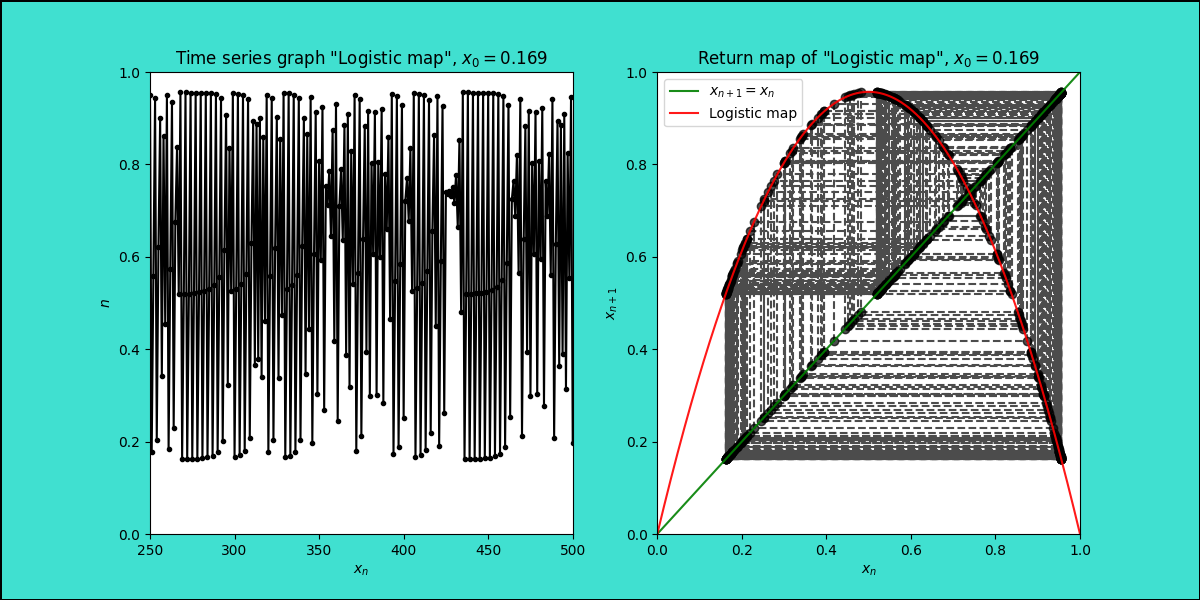
\includegraphics[keepaspectratio, scale=0.5]{images/Problem7/tast7_2.png}
\end{figure}
\subsubsection{考察}
課題1と比較すると $r$ の変化は $0.0001$ なのに対し、時系列グラフとリターンマップには大きな変化が見られた。また、初期値をランダムにとっているため複数回プログラムを実行させた結果、毎回違うグラフが出力された。よって、$r = 3.8284$ のときは、カオスの条件に当てはまると考察した。また課題1の $r$ の値から、$r = 3.8284 と r = 3.8285$ の間に周期倍分岐が起きていることが考察できる。

\subsection{課題3}
\subsubsection{問題}
次に説明する写像 $f^{(3)}$ について、リターンマップを描け(横軸$x_n$, 縦軸$x_{n+3}$)\\
 これまで $x_{n+1} = f \left( x_n \right)$ の写像について考えてきた(ここで関数 $f$ は、上で定義したロジスティック写像)。時系列は $x_0, x_1, x_2, x_3, x_4, x_5, ...$ を順に書いてきたが、上のパラメータでは、だいたいの部分において周期3の運動をしている。そこでここでは、3つ飛ばしで時系列とリターンマップを考える。\\
 いま $x_{n+1} = f \left( x_n \right)$ だから、同様に $x_{n+2} = f \left( x_{n+1} \right), x_{n+3} = f \left( x_{n+2} \right)$ が成り立つ。これらをまとめると、$x_{n+3} = f \left( x_{n+2} \right) = f \left( f \left( x_{n+1} \right) \right) = f \left( f \left( f \left( x_n \right) \right) \right)$と書ける。\\
 この、$x_n$ から $x_{n+3}$ を求める式 $x_{n+3} = f \left( f \left( f \left( x_n \right) \right) \right)$ を簡単のために $x_{n+3} = f^{(3)}\left( x_n \right)$ と書くことにする。これまでは、 $x_n$ と $x_{n+1}$ の間のリターンマップを書いてきたが、$x_n$ と $x_{n+1}$ の間のリターンマップを $r = 3.8284$ のときに書いてみよ。また、下右図のようなリターンマップの階段状にはさまれた部分は何を意味するか考えよ。
\subsubsection{画像}
\begin{figure}[htbp]
  \centering
  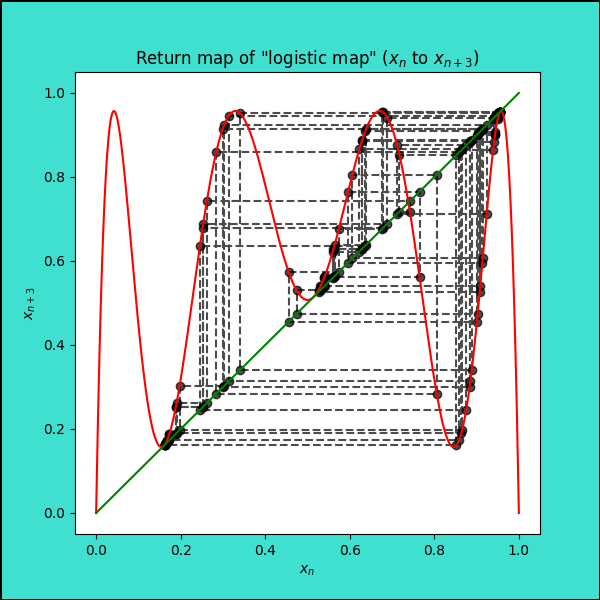
\includegraphics[keepaspectratio, scale=0.5]{images/Problem7/tast7_3.png}
\end{figure}

\subsubsection{考察}
階段上に挟まれた部分はクモの巣図でとっている $x_n$ の時の $x_{n+3}$ の値であると考察した。その理由は範囲が $[0.9561, 0.9565]$ のため曲線の一番右の部分と $x_n = x_{n+3}$ のクモの巣図を拡大しているからである。また、グラフと拡大グラフにより収束したのちに再度発散するような動きになっている。そのため完全には交わっているわけでなく近似していると考察することができる。

\subsubsection{ソースコード}
課題1から課題3までのソースコードを記載している。
\begin{lstlisting}[caption=task7.py]
  from matplotlib import pyplot as plt
  import numpy as np
  from random import uniform


  class Task7():
      def __init__(self) -> None:
          # 初期値 x0 = 0.1
          self.x = uniform(0, 1)
          self.xn = np.linspace(0, 1, 1000)                   # 横軸の範囲と刻み幅
          self.fig = plt.figure(figsize=(12, 6), facecolor='turquoise',
                                linewidth=1, edgecolor='black')

      def logistic(self, r) -> list:
          "リターンマップでのロジスティック写像の座標を持つ配列を返す"
          calc_x = self.x
          x_array = []
          for i in range(1, 501):
              calc_x = r * calc_x * (1 - calc_x)
              if 250 <= i <= 500:
                  x_array.append(calc_x)
          return x_array

      def plot_time_series_graph(self, r: float) -> None:
          "時系列グラフの描画(ロジスティック写像)"
          ax1 = self.fig.add_subplot(1, 2, 1)
          n = list(range(250, 501))
          ax1.plot(n, self.logistic(r), marker='.', color='black')
          ax1.set_title(
              "Time series graph \"Logistic map\", $x_0 = $" + str(round(self.x, 3)))
          ax1.set_xlim(250, 500)
          ax1.set_ylim(0, 1)
          ax1.set_xlabel("$x_n$")
          ax1.set_ylabel("$n$")

      def plot_return_map(self, r) -> None:
          "リターンマップの描画(ロジスティック写像)"
          ax2 = self.fig.add_subplot(1, 2, 2)
          n = self.logistic(r)
          spider_array_x = []                                 # クモの巣図用の配列(x)
          spider_array_y = []                                 # クモの巣図用の配列(y)
          for i in range(1, len(n)):
              spider_array_x.append(n[i - 1])
              spider_array_x.append(n[i])
              spider_array_y.append(n[i])
              spider_array_y.append(n[i])
          logistic_y = []                                     # テント写像のグラフを描くための配列
          for i in self.xn:
              logistic_y.append(r * i * (1 - i))

          ax2.plot(spider_array_x, spider_array_y, marker='o',
                  linestyle='dashed', color='black', alpha=0.7)
          ax2.plot(self.xn, self.xn, color='green',
                  alpha=0.9, label="$x_{n+1} = x_n$")
          ax2.plot(self.xn, logistic_y, color='red',
                  alpha=0.9, label="Logistic map")
          ax2.set_title(
              "Return map of \"Logistic map\", $x_0 = $" + str(round(self.x, 3)))
          ax2.set_xlim(0, 1)
          ax2.set_ylim(0, 1)
          ax2.set_xlabel("$x_n$")
          ax2.set_ylabel("$x_{n+1}$")
          ax2.legend(loc='best')

      def code_problem1(self) -> None:
          r = 3.8285
          self.fig = plt.figure(figsize=(12, 6), facecolor='turquoise',
                                linewidth=1, edgecolor='black')
          self.plot_time_series_graph(r)
          self.plot_return_map(r)
          plt.savefig('複雑系科学演習/Week7/images/task7_1')

      def code_problem2(self) -> None:
          r = 3.8284
          self.fig = plt.figure(figsize=(12, 6), facecolor='turquoise',
                                linewidth=1, edgecolor='black')
          self.plot_time_series_graph(r)
          self.plot_return_map(r)
          plt.savefig('複雑系科学演習/Week7/images/tast7_2')

      def preprocessing(self, x: float) -> float:
          r = 3.8284
          return(r * x * (1 - x))

      def code_problem3(self):
          r = 3.8284
          self.fig = plt.figure(figsize=(6, 6), facecolor='turquoise',
                                linewidth=1, edgecolor='black')

          fff_array_x = []
          fff_array_y = []
          for i in self.xn:
              fff_array_x.append(i)
              fff_array_y.append(self.preprocessing(
                  self.preprocessing(self.preprocessing(i))))

          n = self.logistic(r)
          spider_array_x = []                                 # クモの巣図用の配列(x)
          spider_array_y = []                                 # クモの巣図用の配列(y)
          for i in range(3, len(n), 3):
              spider_array_x.append(n[i - 3])
              spider_array_x.append(n[i])
              spider_array_y.append(n[i])
              spider_array_y.append(n[i])
          plt.plot(spider_array_x, spider_array_y, marker='o',
                  linestyle='dashed', color='black', alpha=0.7)
          plt.plot(fff_array_x, fff_array_y, color='red', label='$Logistic map$')
          plt.plot(self.xn, self.xn, color='green', label='$x_{n+3} = x_n$')
          plt.title('Return map of "logistic map" ($x_n$ to $x_{n+3}$)')
          plt.xlabel('$x_n$')
          plt.ylabel('$x_{n+3}$')
          plt.savefig('複雑系科学演習/Week7/images/tast7_3')


  task = Task7()
  task.code_problem1()
  task.code_problem2()
  task.code_problem3()
\end{lstlisting}

\subsection{課題4}
$x_{n+1} = f \left( x_n \right)$ である時、$x_{n+2} = f \left( x_{n+1} \right), x_{n+3} = f \left( x_{n+2} \right)$ である。従って、$x_{n+3} = f \left( f \left( x_{n+1} \right) \right) = f \left( f \left( f \left( x_n \right) \right) \right)$と書ける。$y = f \left( f \left( f \left( x_n \right) \right) \right)$ のグラフを描き、この曲線が $y = x$ と区間 $[0, 1]$ において互いに異なる3つの点で接する時の $r$ の値は、$r = 1 + \sqrt{8}$ であることをグラフを描いて確認せよ。
\subsubsection{画像}
\begin{figure}[htbp]
  \centering
  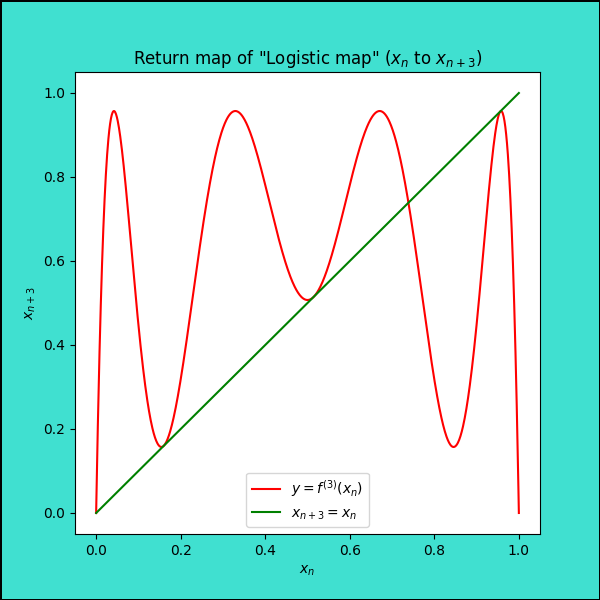
\includegraphics[keepaspectratio, scale=0.5]{images/Problem7/tast7_4.png}
\end{figure}

\subsubsection{考察}
画像から、$r = 1 + \sqrt{8} のとき y = f^{(3)} \left( x_n \right) と x_{n+1} = x_n$ は3点で接していると確認することができる。また、課題3の挟まれた部分のグラフを見ると、$r = 3.8284$ のときには$y = f^{(3)} \left( x_n \right) と x_{n+1} = x_n$ は接することなく収束したのち発散していることが読み取れる。さらに、$1 + \sqrt{8} = 3.82842712474...$ である。以上のことから、$r = 1 + \sqrt{8}$ を境に3周期の特徴を持つと考察することができる。

\subsubsection{ソースコード}
\begin{lstlisting}[caption=task7-4.py]
  from matplotlib import pyplot as plt
  import numpy as np
  from random import uniform


  class Week7Task4():
      def __init__(self) -> None:
          self.x = uniform(0, 1)
          self.r = 1 + 8**(1 / 2)
          self.xn = np.linspace(0, 1, 1000)
          self.fig = plt.figure(figsize=(6, 6), facecolor='turquoise',
                                linewidth=1, edgecolor='black')

      def preprocessing(self, x: float) -> float:
          """前処理"""
          return(self.r * x * (1 - x))

      def code_problem4(self):
          """r = 1 + √8のときのグラフ"""

          fff_array_x = []
          fff_array_y = []
          for i in self.xn:
              fff_array_x.append(i)
              fff_array_y.append(self.preprocessing(
                  self.preprocessing(self.preprocessing(i))))
          plt.plot(fff_array_x, fff_array_y, color='red',
                  label='$y = f^{(3)}(x_n)$')
          plt.plot(self.xn, self.xn, color='green', label='$x_{n+3} = x_n$')
          plt.title('Return map of "Logistic map" ($x_n$ to $x_{n+3}$)')
          plt.xlabel('$x_n$')
          plt.ylabel('$x_{n+3}$')
          plt.legend(loc='best')
          plt.savefig('複雑系科学演習/Week7/images/tast7_4')


  task = Week7Task4()
  task.code_problem4()
\end{lstlisting}

\subsection{課題5}
\subsubsection{問題}
4の結果から $r$ の値が $r = 1 + \sqrt{8}$ より大きい場合と小さい場合において、$x_{n+1} = f \left( x_n \right)$ の安定固定点が幾つあるか理由を述べて答えよ。
\subsubsection{考察}
前回のレポート課題3であるロジスティック写像の分岐図を見て考察した。その結果、$r > 1 + \sqrt{8}$ の場合は3周期をもつときとカオスの状態のときの2つの場合があることが読み取れる。具体的には、$r = 1 + \sqrt{8}$ から進むにつれ周期倍分岐を起こし、その後カオスの状態へと変化していく。よって、安定固定点は$3, 6, ...$ と変化していくと考察した。また、$r < 1 + \sqrt{8}$ の場合は、カオスの状態になるため安定固定点はないと考察した。

\subsection{課題6}
\subsubsection{問題}
4,5から $r = 1 + \sqrt{8}$ の場合に生じたラミナーとバーストは$x_{n+3} = f \left( f \left( f \left( x_n \right) \right) \right)$ の値と $x_n$ の値がどのように変化する時に現れる現象であるか説明せよ。
\subsubsection{考察}
複数回実行するとラミナーとバーストの周期性は捉えることができなかった。

\section{レポート課題 3rd}
\subsection{課題1}
\subsubsection{問題}
$a = 1.4, b = 0.3$ として、Henon写像のアトラクタを描け。アトラクタへ至るまでの過渡状態は書かなくてよい。
\subsubsection{画像}
\begin{figure}[htbp]
  \centering
  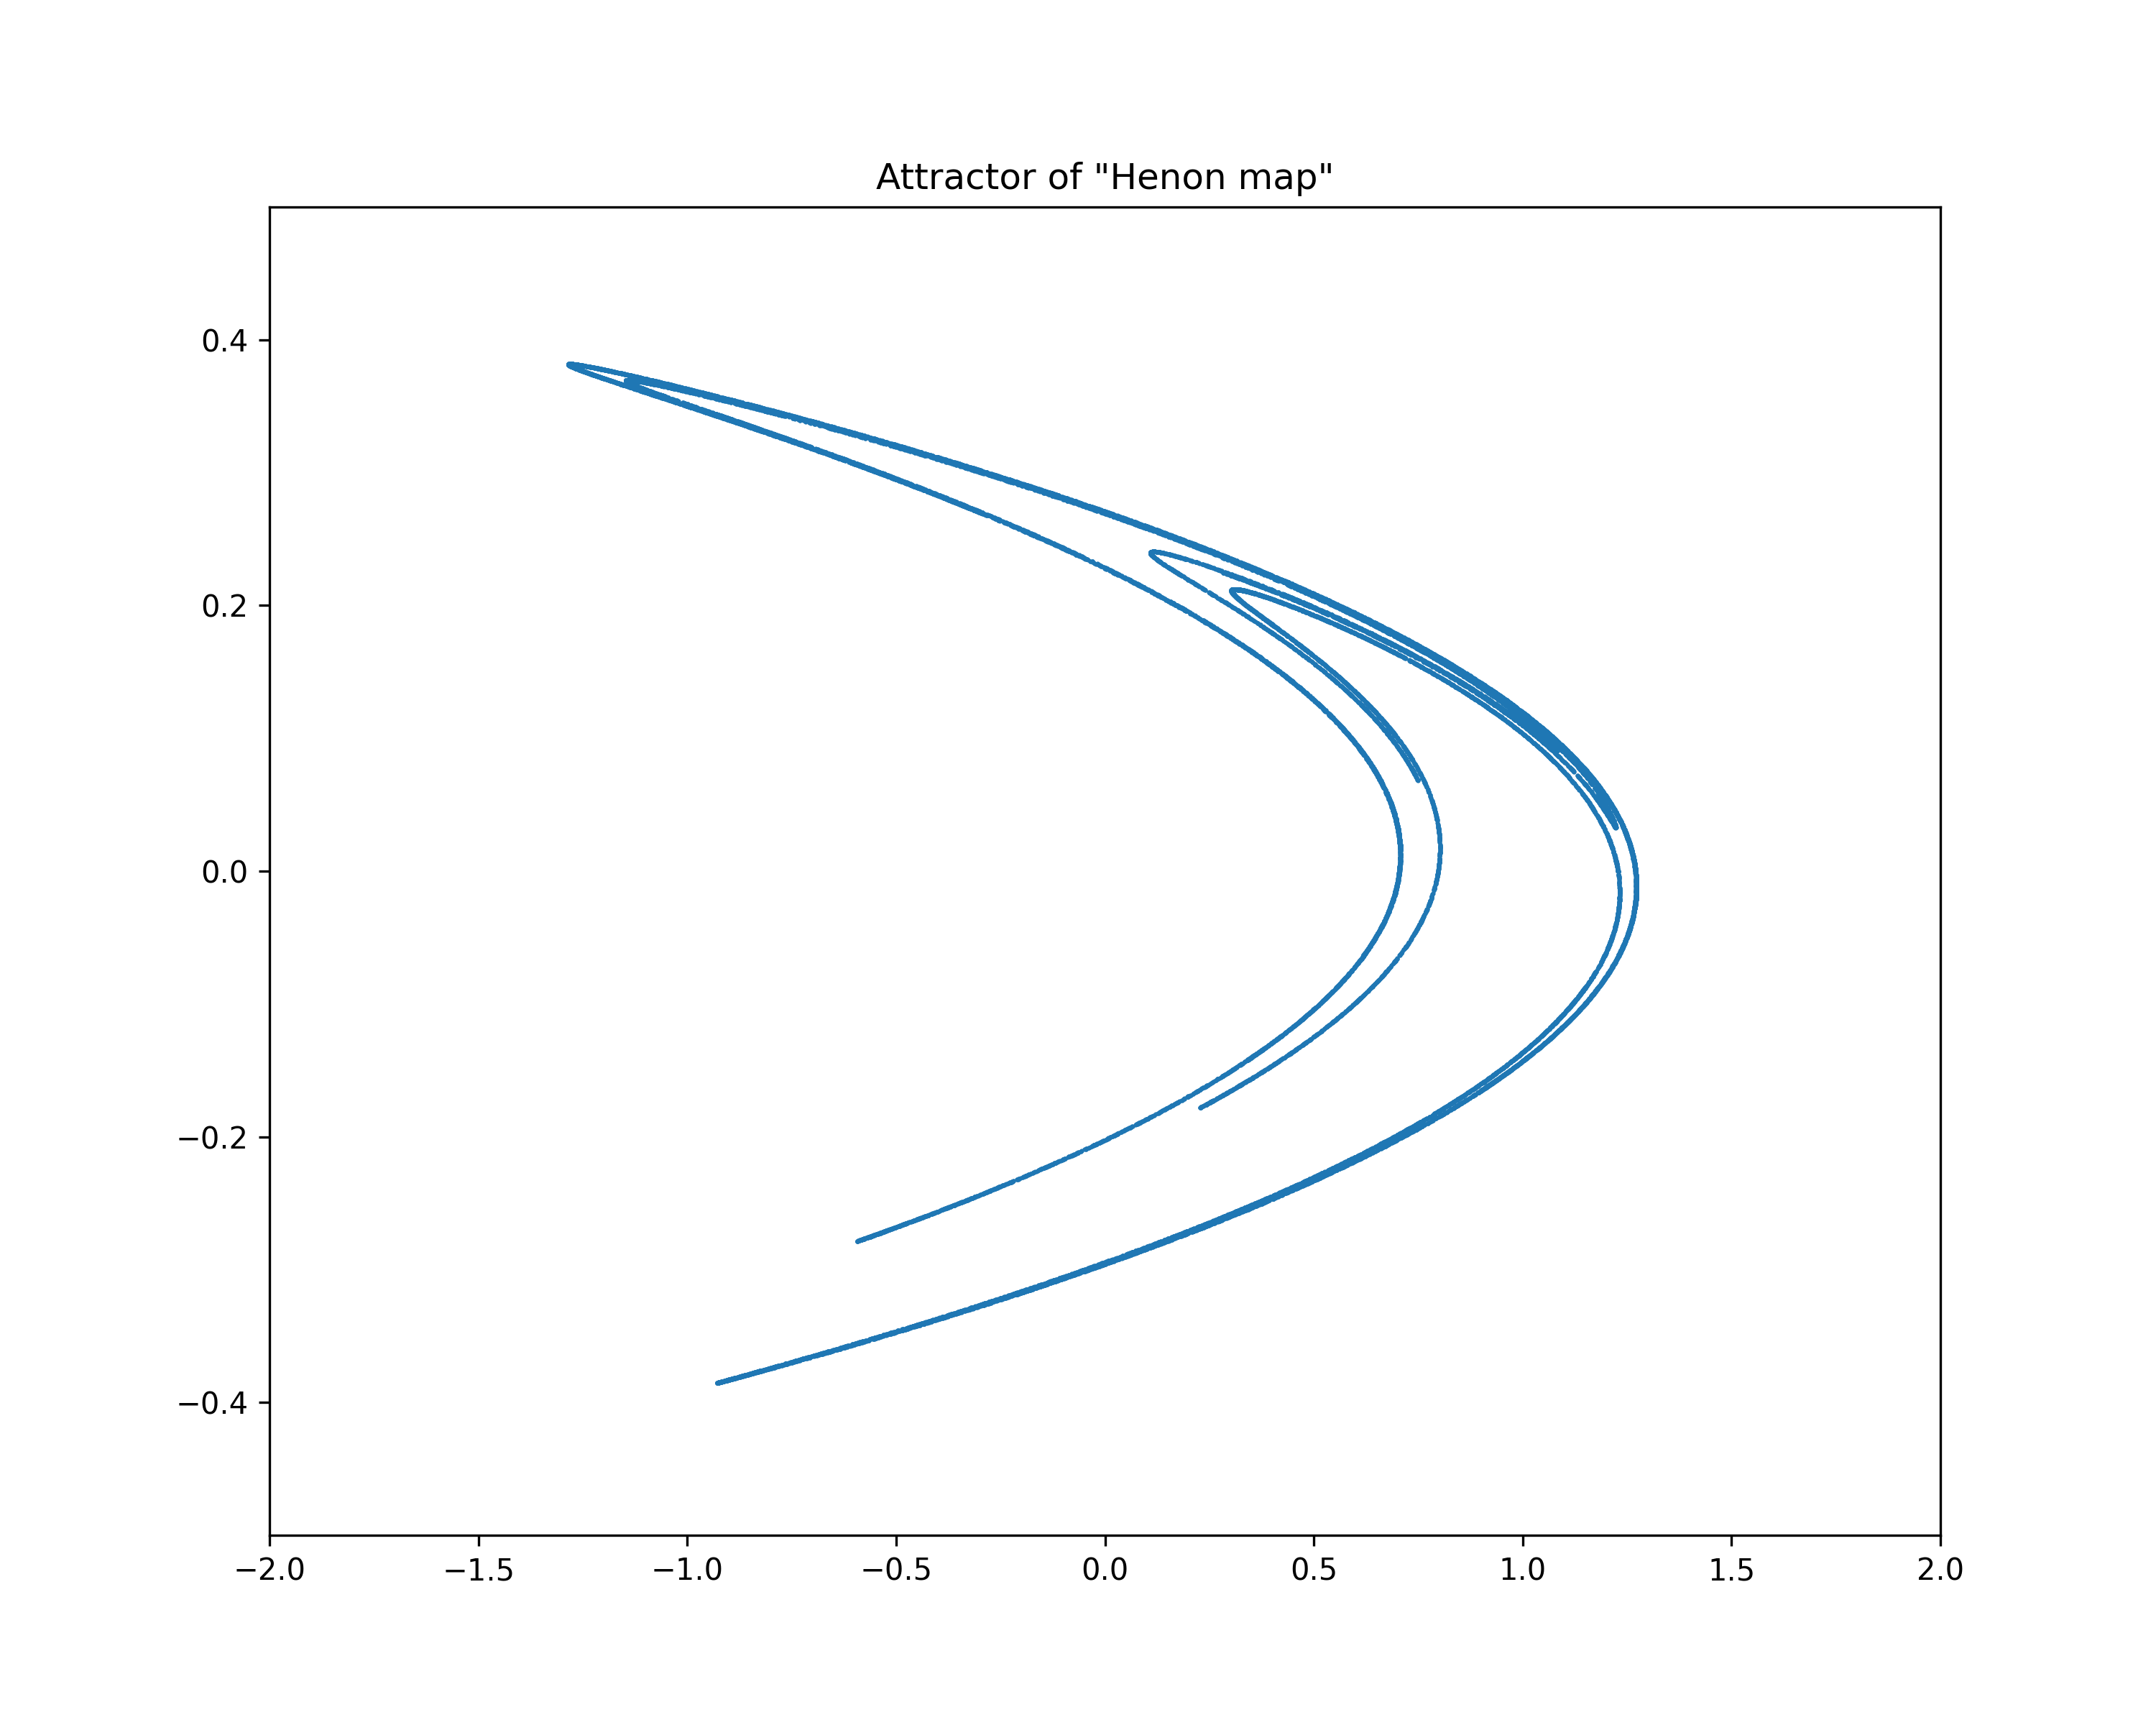
\includegraphics[keepaspectratio, scale=0.5]{images/Problem8/task8_1.png}
\end{figure}
\subsubsection{考察}
漸化式を代入しPythonで実行させた結果、画像のような結果になった。この画像を拡大していくと同様の解軌道を描いていくことが発見できた。そのため、エノン写像にはフラクタル構造があるのではないかと考察した。
\subsubsection{ソースコード}
\begin{lstlisting}[caption=task8-1.py]
  from matplotlib import pyplot as plt
  from random import uniform


  def henon(x: float, y: float):
      return y + 1 - a * x ** 2, b * x


  x = uniform(-1, 1)
  y = uniform(-1, 1)
  a = 1.4
  b = 0.3
  cnt = 30000
  x_array = []
  y_array = []
  for i in range(cnt):
      x, y = henon(x, y)
      if i < 249:
          continue
      x_array.append(x)
      y_array.append(y)
  plt.figure(figsize=(10, 8))
  plt.plot(x_array, y_array, linestyle='None', marker='.', markersize=1)
  plt.title('Attractor of "Henon map"')
  plt.xlim(-2, 2)
  plt.ylim(-0.5, 0.5)
  # plt.show()
  plt.savefig('複雑系科学演習/Week8/images/task8_1', dpi=300)
\end{lstlisting}

\newpage
\subsection{課題2}
\subsubsection{問題}
$b = 0.3$ に固定して、横軸 $a$ 縦軸 $x_n$ の分岐図を描け。$a \in [0, 1.5]$ を $0.01$ 刻みで変化させたときの、$x_n(n = 250から500)$ の点を打つこと。時間とファイルサイズが許すなら、より刻み幅を小さくしてもよい。
\subsubsection{画像}
\begin{figure}[htbp]
  \centering
  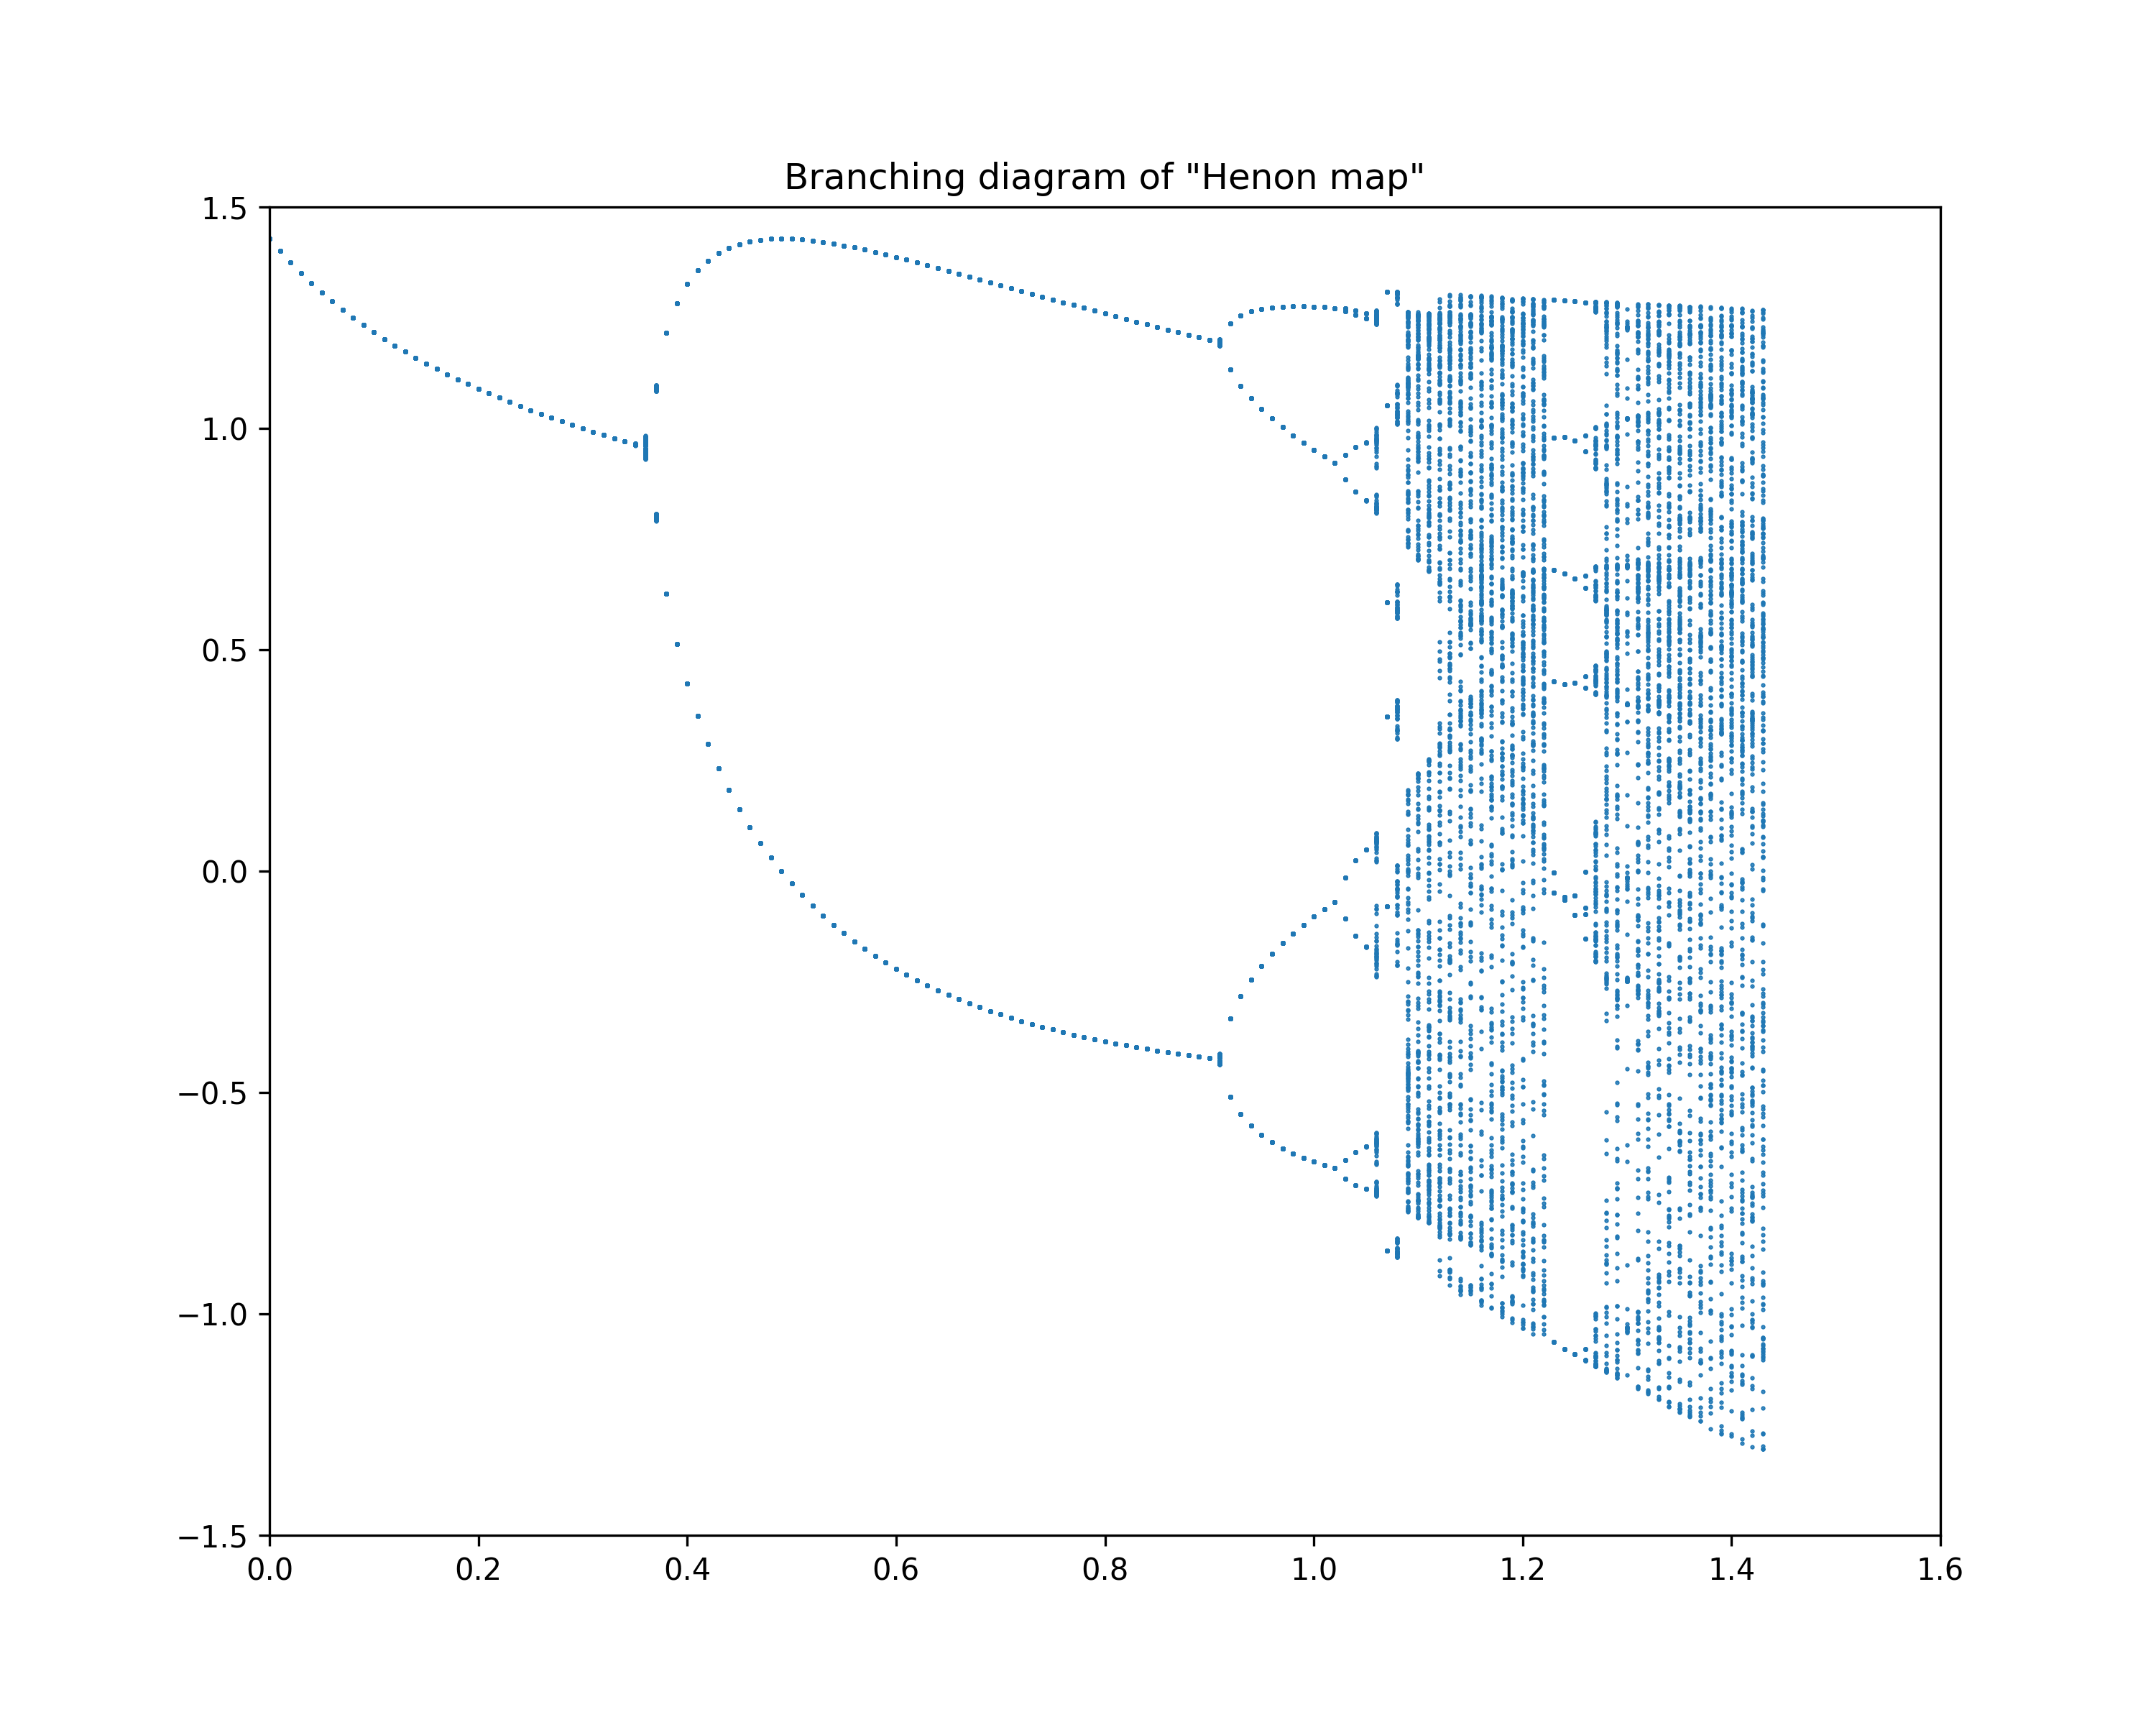
\includegraphics[keepaspectratio, scale=0.5]{images/Problem8/task8_2.png}
\end{figure}
\subsubsection{考察}
考察については次の課題3に記述している。

\subsubsection{ソースコード}
\begin{lstlisting}[caption=task8-2.py]
  from matplotlib import pyplot as plt
  import numpy as np
  from random import uniform


  def henon(a: float, x: float, y: float):
      """エノン写像の(x, y)座標を返す関数"""
      return y + 1 - a * x ** 2, b * x


  a = np.arange(0, 1.5, 0.01, dtype=object)   # 課題2の a の範囲
  b = 0.3                                     # b = 0.3 に固定
  x0 = uniform(-1, 1)                         # ランダムの初期値x0([-1, 1]の範囲)
  y0 = uniform(-1, 1)                         # ランダムの初期値y0([-1, 1]の範囲)
  x_array = []                                # x の値を保存するための配列
  a_array = []                                # a の値を保存するための配列

  for i in a:                                 # 各 a のときの振る舞いを計算する
      x = x0
      y = y0
      for j in range(500):
          x, y = henon(i, x, y)
          if x < -1.5 or 1.5 < x:             # プロットの範囲外なら終了(オーバーフローを避けるため)
              break
          if j < 249:                         # 250 < xn < 500 の範囲外なら配列に入れない
              continue
          x_array.append(x)
          a_array.append(i)

  plt.figure(figsize=(10, 8))
  plt.plot(a_array, x_array, linestyle='None', marker='.', markersize=1)
  plt.title('Branching diagram of "Henon map"')
  plt.xlim(0, 1.6)
  plt.ylim(-1.5, 1.5)
  # plt.show()
  plt.savefig('複雑系科学演習/Week8/images/task8_2', dpi=300)
\end{lstlisting}

\subsection{課題3}
\subsubsection{問題}
問2の分岐図よりわかることは何か?(例えば分岐の種類など)
\subsubsection{考察}
$r = 0.4$ 付近を境に周期倍分岐を起こしていることが読み取れた。
\section{レポート課題4}
\subsection{課題1}
\subsubsection{問題}
$10 \times 10$ 分割したマス目内にアトラクタの点が入っているかどうか調べる。点が入っているマス目の数を数えよ。
\subsubsection{解答と考察}
実際にレポート課題4の下にある参考ソースコードを埋め実行してみた。すると[10 34]が出力結果として出てきた。そのためマス目の数は34個である。ソースコードは$N = 1, 2, ..., 500$ までの結果を一括で表示したため最後に掲載する。

\subsection{課題2}
\subsubsection{問題}
$50 \times 50, 100 \times 100, 500 \times 500$ 分割したとき、同様の手順でアトラクタの点が入っているマス目を(プログラムを用いて)数えよ。
\subsubsection{解答と考察}
同様に $N = 50, 100, 500$ で実行した。その結果[50 254], [100 604], [500 4290]がそれぞれ出力された。よってマス目の数は、
\begin{itemize}
  \item $N = 50$ のとき254個
  \item $N = 100$ のとき604個
  \item $N = 500$ のとき4290個
\end{itemize}
となった。また、ソースコードは$N = 1, 2, ..., 500$ までの結果を一括で表示したため最後に掲載する。

\newpage
\subsection{課題3}
\subsubsection{問題}
$N \times N$ 分割したとき上で得た結果が $m \left( N \right)$ だったとする。横軸 $N$ 、縦軸 $m \left( N \right)$ として両対数グラフを描け。何がわかるか。
\subsubsection{画像}
\begin{figure}[htbp]
  \centering
  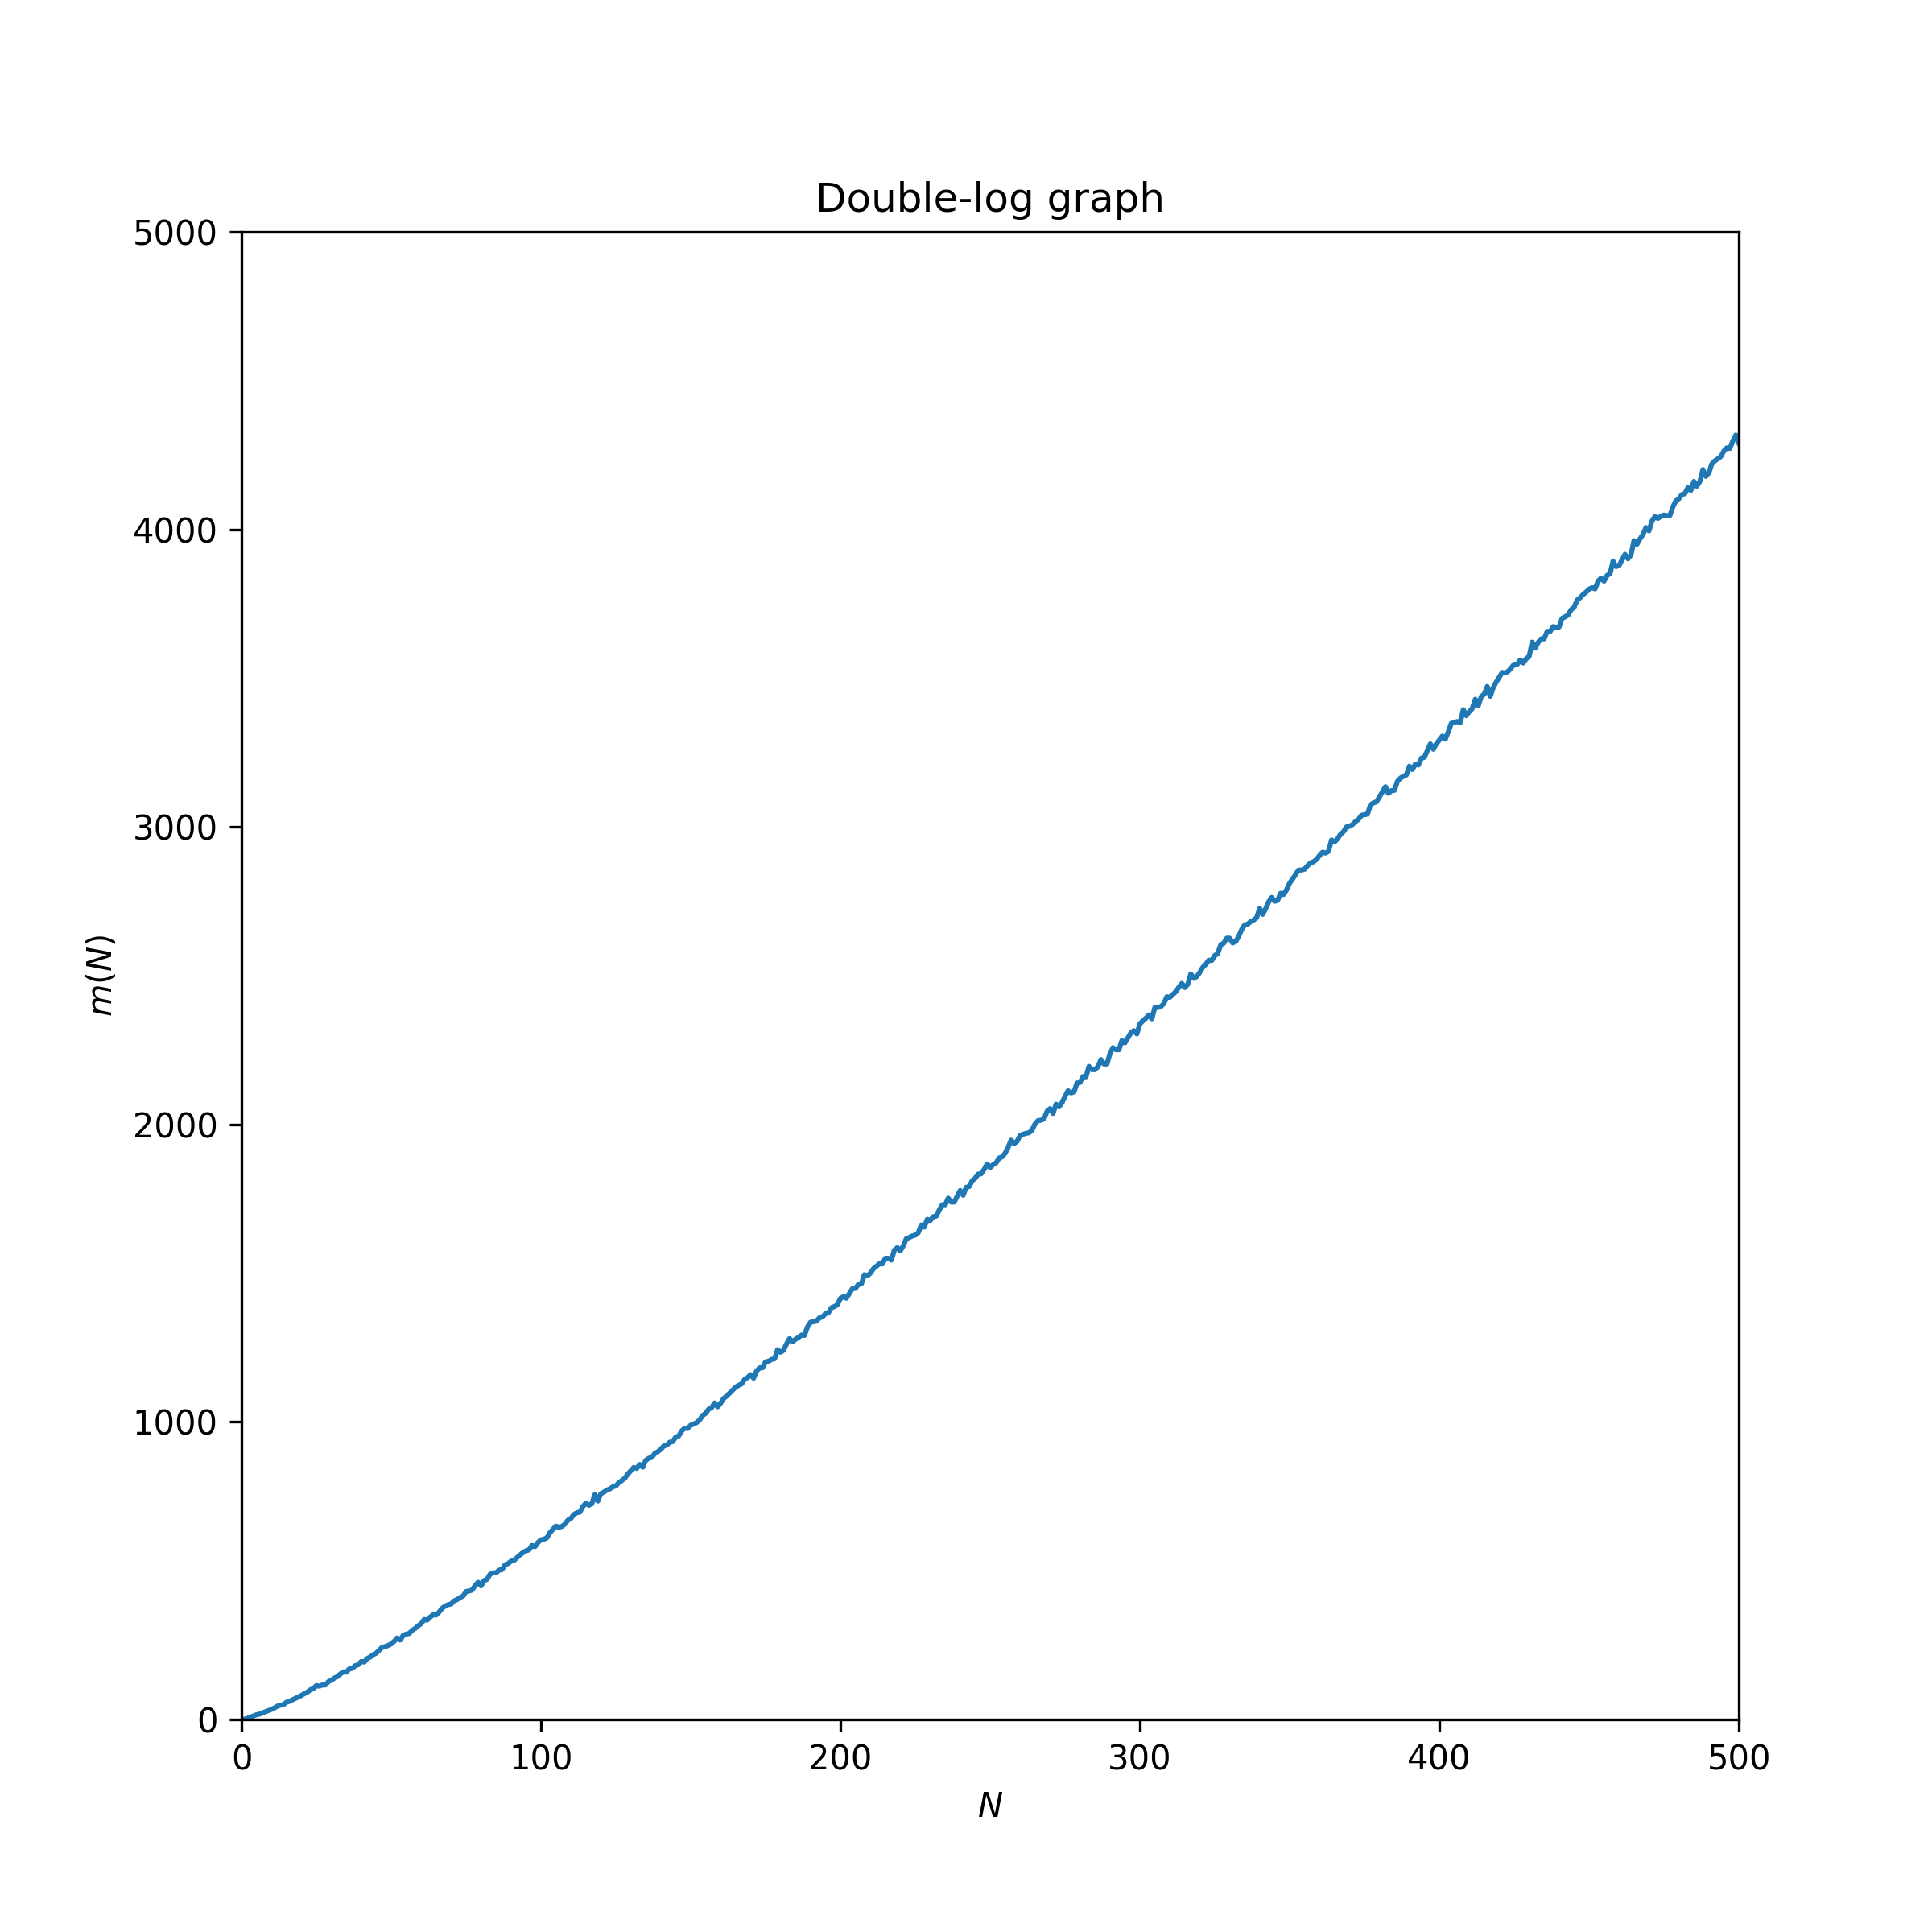
\includegraphics[keepaspectratio, scale=0.5]{images/Problem9/task9.png}
\end{figure}

\subsubsection{考察}
Pythonでは、それぞれの個数を計算するときの計算量に問題があったため、今回は個数計算をC言語グラフの描画をPythonで行った。考察としては、最初のみ直線とは違うような増加の仕方をするが、$N = 50$ あたり以降からは直線的な増加をしていることが挙げられる。


\subsubsection{ソースコード}
\begin{lstlisting}[caption=ctest9.c]
  #include <stdio.h>
  #define N 1000000
  #define nSizeMax 1000

  #define xmin -1.5
  #define xmax 1.5
  #define ymin -0.5
  #define ymax 0.5

  int hist[nSizeMax][nSizeMax];

  void next(double* x, double* y, double a, double b) {
      double xx = (*y) + 1 - a * (*x) * (*x);
      double yy = b * (*x);
      *x = xx;
      *y = yy;
  }

  // initialization
  void init(int nS) {
      int i, j;
      for ( i = 0; i < nS; i++ ) {
          for ( j = 0; j < nS; j++ ) {
              hist[i][j] = 0;
          }
      }
  }

  // print out
  void print(int nS) {
      int i, j, count = 0;
      for ( i = 0; i < nS; i++ ) {
          for ( j = 0; j < nS; j++ ) {
              if (hist[i][j]) {
                  count++;
              }
          }
      }
      printf("%d %d\n", nS, count);
  }


  int main(){
      double a = 1.4, b = 0.3;
      double x = 0.5, y = 0.5;

      for (int nSize = 0; nSize <= 500; nSize++) {
          init(nSize);
          int px, py;
          for (int n = 0; n <= N; n++) {
              next(&x, &y, a, b);
              if (n > 10000) {
                  px = (int)((x - xmin) / (xmax - xmin) * nSize);
                  py = (int)((y - ymin) / (ymax - ymin) * nSize);
                  hist[px][py] = 1;
              }
          }
          print(nSize);
      }
      return 0;
  }
\end{lstlisting}

\begin{lstlisting}[caption=task9.py]
  from matplotlib import pyplot as plt
  import numpy as np

  filepath = '複雑系科学演習/Week9/ctest9.txt'
  x_array = []
  y_array = []
  with open(filepath, encoding='UTF-8') as f:
      while line := f.readline():
          line = line.rstrip()
          x, y = line.split(' ')
          x_array.append(int(x))
          y_array.append(int(y))

  plt.figure(figsize=(8, 8))
  plt.xlim(0, 500)
  plt.ylim(0, 5000)
  plt.plot(x_array, y_array)
  plt.title('Double-log graph')
  plt.xlabel('$N$')
  plt.ylabel('$m(N)$')
  # plt.show()
  plt.savefig('複雑系科学演習/Week9/images/task9', dpi=300)
\end{lstlisting}
\end{document}